\documentclass{cmc}

\begin{document}

\pagestyle{fancy}
\lhead{\textit{\textbf{Computational Motor Control, Spring 2019} \\
    Python exercise, Lab 6, GRADED}} \rhead{Students \\ Honigmann, Munier \& Plett Palomar}

\section*{Student names: Honigmann Simon, Munier Louis \& Plett Palomar Kilian Asterio}
\textit{Instructions: Update this file (or recreate a similar one,
  e.g.\ in Word) to prepare your answers to the questions. Feel free
  to add text, equations and figures as needed. Hand-written notes,
  e.g.\ for the development of equations, can also be included e.g.\
  as pictures (from your cell phone or from a scanner).
  \textbf{\corr{This lab is graded.}} and must be submitted before
  the \textbf{\corr{Deadline : 11-04-2018 Midnight}}.  \\ Please
  submit both the source file (*.doc/*.tex) and a pdf of your
  document, as well as all the used and updated Python functions in a
  single zipped file called \corr{lab6\_name1\_name2\_name3.zip} where
  name\# are the team member’s last names.  \corr{Please submit only
    one report per team!}}
\\

\textit{The file \fileref{lab\#.py} is provided to run all exercises
  in Python.
  % Each \fileref{exercise\#.py} can be run to run an exercise
  % individually.
  The list of exercises and their dependencies are shown in
  Figure~\ref{fig:files_lab6}.
  When a file is run, message logs will be printed to indicate
  information such as what is currently being run and and what is left
  to be implemented. All warning messages are only present to guide
  you in the implementation, and can be deleted whenever the
  corresponding code has been implemented correctly.}


% \textit{In this exercise, you will explore the different modeling
%   techniques that can be used to control a single joint and
%   segment. We initially start by exploring a single joint controlled
%   by a pair of antagonist spring like muscles and then extend the
%   model by adding dampers to it. These only represent the passive
%   dynamics observed in a real musculoskeletal system. To make the
%   behavior more realistic we then study more complex hill muscle model
%   in detail. }

\begin{figure}[ht]
  \centering 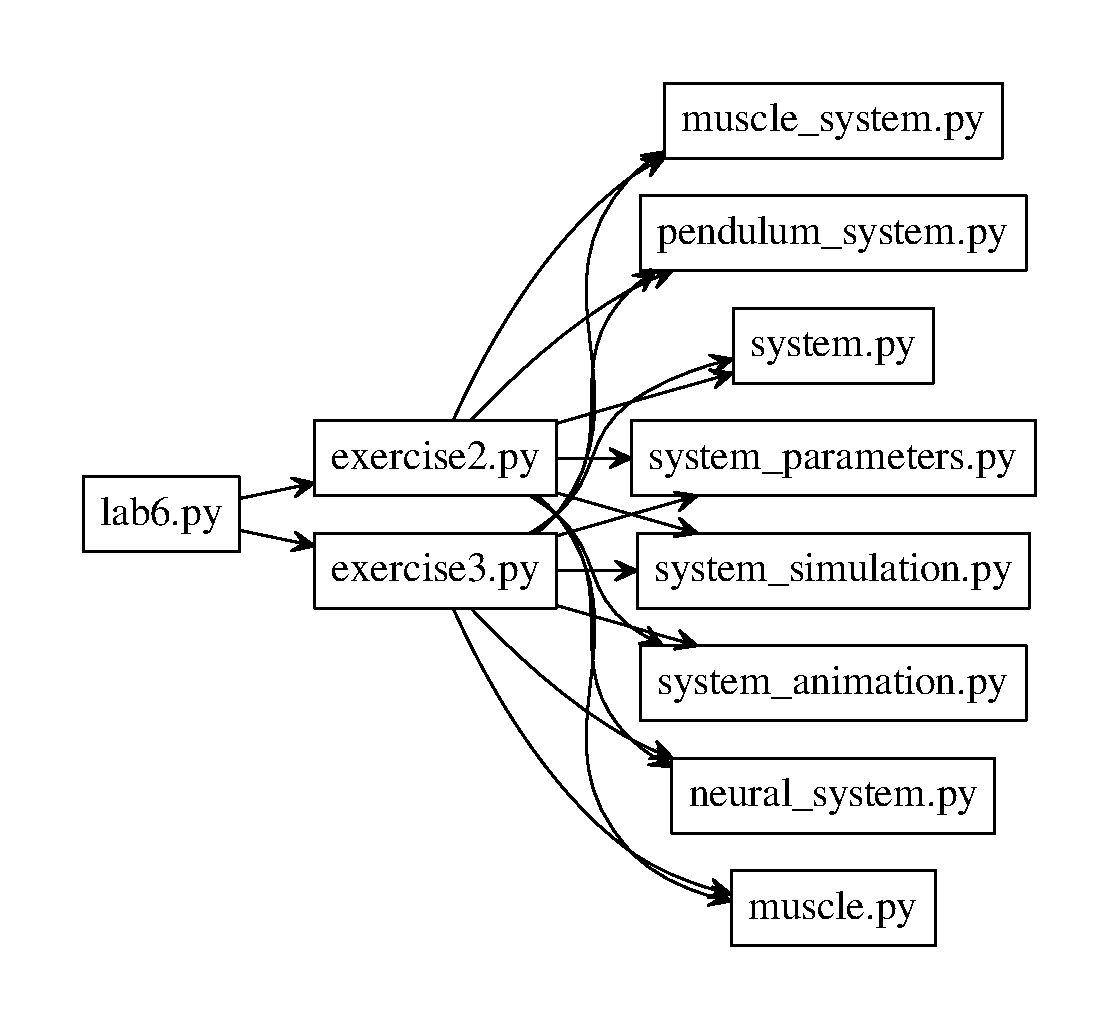
\includegraphics[width=0.5\textwidth]{figures/files_lab6}
  \caption{\label{fig:files_lab6} Exercise files dependencies. In this lab,
    you will be modifying \fileref{exercise1.py} and
    \fileref{pendulum\_system.py}}
\end{figure}

\subsection*{Files to complete the exercises}
\label{sec:intro_lab6}

\begin{itemize}
\item \fileref{lab6.py} : Main file
\item \fileref{exercise2.py} : Main file to complete exercise 2
\item \fileref{exercise3.py} : Main file to complete exercise 3
\item \fileref{system\_parameters.py} : Parameter class for Pendulum,
  Muscles and Neural Network (Create an instance and change properties
  using the instance. You do not have to modify the file)
\item \fileref{muscle.py} : Muscle class (You do not have to modify
  the file)
\item \fileref{system.py} : System class to combine different models %
  like Pendulum, Muscles, Neural Network (You do not have to modify
  the file)
\item \fileref{pendulum\_system.py} : Contains the description of
  pendulum equation and Pendulum class. You can use the file to define
  perturbations in the pendulum.
\item \fileref{muscle\_system.py} : Class to combine two muscles (You
  do not have to modify the file)
\item \fileref{neural\_system.py} : Class to describe the neural
  network (You do not have to modify the file)
\item \fileref{system\_simulation.py} : Class to initialize all the
  systems, validate and to perform integration (You do not have to
  modify the file)
\item \fileref{system\_animation.py} : Class to produce animation of
  the systems after integration (You do not have to modify the file)
\end{itemize}

\textbf{NOTE : } '\textit{You do not have to modify}' does not mean
you should not, it means it is not necessary to complete the
exercises. But, \corr{you are expected to look into each of these
  files and understand how everything works}. You are free to explore
and change any file if you feel so.

\section*{Exercise 2 : Pendulum model with Muscles}
\label{sec:question-1}

\begin{figure}[H]
  \centering 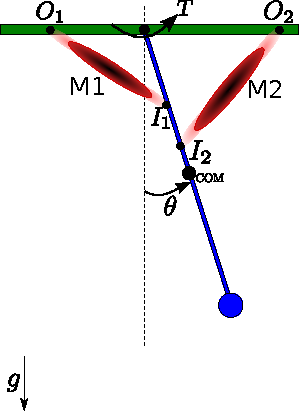
\includegraphics[scale=1.0]{figures/pendulum_muscles.pdf}
  \caption{Pendulum with Antagonist Hill Muscles}
  \label{fig:p_muscles}
\end{figure}

The system is comprised of a physical pendulum described by equation
\ref{eq:pendulum} and a pair of antagonist muscles \textbf{M1} and
\textbf{M2}. Muscle \textbf{M1} extends the pendulum ($\theta$
increases) and Muscle \textbf{M2} flexes the muscle ($\theta$
decreases).

Consider the system only for the pendulum range $\theta$ =
$[-\pi/2, \pi/2]$

\begin{equation}
  \label{eq:pendulum}
  I\ddot{\theta} = -0.5 \cdot m \cdot g \cdot L \cdot sin(\theta)
\end{equation}

Where,

\begin{itemize}
\item $I$ - Pendulum inertia about the pendulum pivot joint
  [$kg \cdot m^2$]
\item $\theta$ - Pendulum angular position with the vertical [$rad$]
\item $\ddot{\theta}$ - Pendulum angular acceleration
  [$rad \cdot s^{-2}$]
\item $m$ - Pendulum mass [$kg$]
\item $g$ - System gravity [$m \cdot s^{-2}$]
\item $L$ - Length of the pendulum [$m$]
\end{itemize}

Each muscle is modelled using the Hill-type equations that you are now
familiar with.  Muscles have two attachment points, one at the origin
and the other at the insertion point.  The origin points are denoted
by $O_{1,2}$ and the insertion points by $I_{1,2}$. The two points of
attachment dictate how the length of the muscle changes with respect
to the change in position of the pendulum.

The active and passive forces produced by the muscle are transmitted
to the pendulum via the tendons. In order to apply this force on to
the pendulum, we need to compute the moment based on the attachments
of the muscle.

Using the laws of sines and cosines, we can derive the length of
muscle and moment arm as below. The reference to the paper can be
found here
\href{https://www.ncbi.nlm.nih.gov/pmc/articles/PMC5323435}{\corr{Reference}},

\begin{eqnarray}
  \label{eq:2_lab6}
  L_1 = \sqrt[2]{a_{1}^2 + a_{2}^2 + 2 \cdot a_1 \cdot a_2 \cdot \sin(\theta)} \\
  h_1 = \frac{a_1 \cdot a_2 \cdot \cos(\theta)}{L_1}
\end{eqnarray}

Where,

\begin{itemize}
\item $L_1$ : Length of muscle 1
\item $a_1$ : Distance between muscle 1 origin and pendulum origin
  ($|O_1C|$)
\item $a_2$ : Distance between muscle 1 insertion and pendulum origin
  ($|I_1C|$)
\item $h_1$ : Moment arm of the muscle
\end{itemize}

\begin{figure}[H]
  \centering
  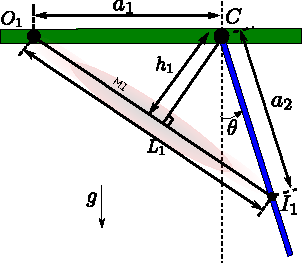
\includegraphics[scale=1]{figures/pendulum_muscles_force_length.pdf}
  \caption[force\_length]{Computation of muscle length and moment arm}
  \label{fig:pendulum_muscles_force_length}
\end{figure}

Equation \ref{eq:2_lab6} can be extended to the Muscle 2 in similar
way. Thus, the final torque applied by the muscle on to the pendulum
is given by,

\begin{equation}
  \label{eq:3}
  \tau = F \cdot h
\end{equation}

Where,

\begin{itemize}
\item $\tau$ : Torque [$N \cdot m$]
\item $F$ : Muscle Tendon Force [$N$]
\item $h$ : Muscle Moment Arm [$m$]

\end{itemize}

In this exercise, the following states of the system are integrated
over time,

\begin{equation}
  \label{eq:6_lab6}
  X = \begin{bmatrix}
    \theta & \dot{\theta} & A_1 & l_{CE1} & A_2 & l_{CE2}
  \end{bmatrix}
\end{equation}

Where,

\begin{itemize}
\item $\theta$ : Angular position of the pendulum [rad]
\item $\dot{\theta}$ : Angular velocity of the pendulum [rad/s]
\item $A_1$ : Activation of muscle 1 with a range between [0, 1].  0
  corresponds to no stimulation and 1 corresponds to maximal
  stimulation.
\item $l_{CE1}$ : Length of contractile element of muscle 1
\item $A_2$ : Activation of muscle 2 with a range between [0, 1].  0
  corresponds to no stimulation and 1 corresponds to maximal
  stimulation.
\item $l_{CE2}$ : Length of contractile element of muscle 2
\end{itemize}

To complete this exercise you will make use of the following files,
\fileref{exercise2.py}, \fileref{system\_parameters.py},
\fileref{muscle.py}, \fileref{system.py}, \fileref{pendulum\_system.py},
\fileref{muscle\_system.py}, \fileref{system\_simulation.py} %

\label{sec:questions}

\subsection*{2a. For a given set of attachment points, compute and
  plot the muscle length and moment arm as a function of $\theta$
  between $[-\pi/4, \pi/4]$ using equations in \corr{eqn:\ref{eq:2_lab6}}
  and discuss how it influences the pendulum resting position and the
  torques muscles can apply at different joint angles. You are free to implement
this code by yourself as it does not have any other dependencies.}
\label{sec:2a}

The figures below show the relationship between angle and muscle length or moment arm. The simulated pendulum's muscles are approximately 24 cm long, each mounted at 45 degrees to the vertical. The muscles are unstretched when the pendulum angle is 0. All other parameters remain as default values (e.g. $l_{pendulum}=50cm, m_{pendulum}=1kg$).

\begin{figure}[H]
    \centering
    \begin{subfigure}[t]{0.49\textwidth}
        \centering
        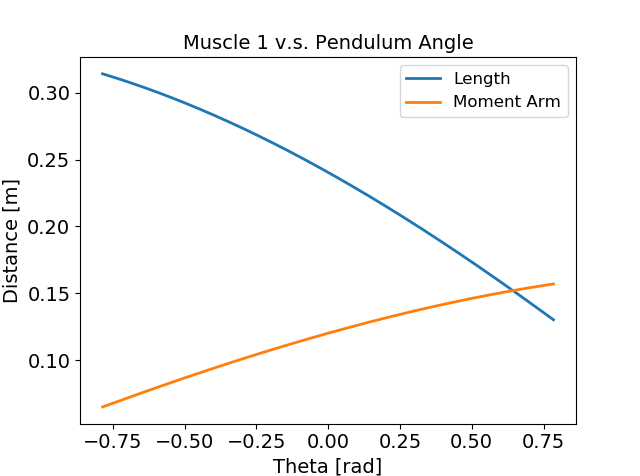
\includegraphics[width=\textwidth]{2a/2a_m1.png}
        \caption{Angle vs Muscle 1 Length and Moment Arm. Muscle 1 has a negative moment arm, but it is plotted as a positive value here to allow for direct comparison with muscle 2.}
    \end{subfigure}
    \hfill
    \begin{subfigure}[t]{0.49\textwidth}
        \centering
        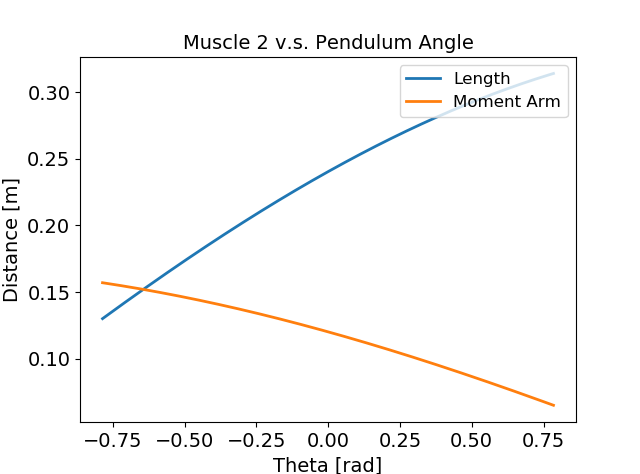
\includegraphics[width=\textwidth]{2a/2a_m2.png}
        \caption{Angle vs Muscle 2 Length and Moment Arm.}
        \end{subfigure}
    \caption{Effect of Pendulum Angle on Muscles}
    \label{fig:2a}
\end{figure}

\begin{figure}[H]
    \centering
    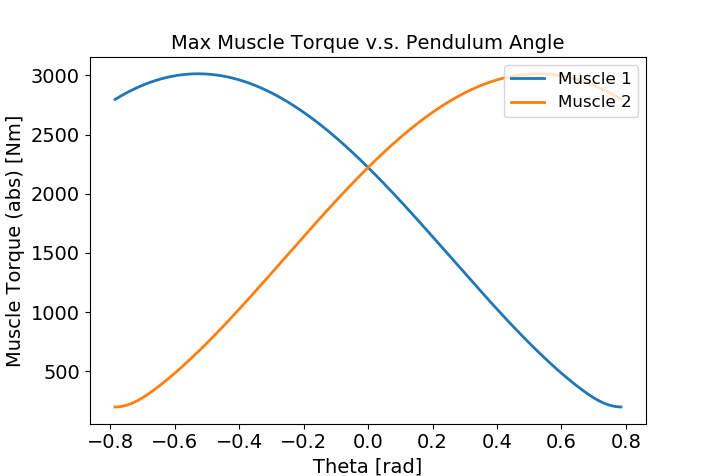
\includegraphics[width=.6\textwidth]{2a/2a_torque.png}
    \caption{Pendulum Angle vs Maximum Muscle Torque ($v_ce = 0$, Stimulation = 1).\\ 
    Muscle 1 produces negative torques, which were plotted as positive values to allow direct comparison.}
    \label{fig:2aTorque}
\end{figure}

From figure \ref{fig:2a}, it can be noted that the muscles are balanced when the angle is equal to 0 and the pendulum is vertical. Both muscles, having the same properties, have the same length and equal and opposite moment arms, resulting in a net-zero torque on the pendulum.\\

The torque applied by each muscle is related to the moment arm, and is related to the muscle force, which is in-turn dependent on muscle length. As the muscle length stretches or contracts from the optimal length, it's force capacity decreases. As the muscle gets shorter, this effect is offset by an increasing moment arm. As the muscle lengthens, the moment arm actually decreases for this configuration. As a result, either muscle will be capable of dominating the other when it is allowed to contract first (all other parameters being equal). \ref{fig:2aTorque} demonstrates this behaviour, with a peak muscle torque occurring at a pendulum angle of about 35 deg (0.6 rad). When the pendulum is pulled to either side, the muscle which has contracted must counter the torque created by the gravitational pull on the pendulum and the torque created by the other muscle. 

\subsection*{2b. Using simple activation wave forms (example : sine or
  square waves) applied to muscles (use
  \fileref{system\_simulation.py::add\_muscle\_activations} method in
  \fileref{exercise2.py}), try to obtain a limit cycle behavior for
  the pendulum. Use relevant plots to prove the limit cycle behavior.
  Explain and show the activation wave forms you used. Use
  \newline \fileref{pendulum\_system.py::PendulumSystem::pendulum\_system} function to perturb the model.}
  
  In this section, a sinusoidal input was applied to each muscle to result in a stable limit cycle behaviour of the pendulum. A 0.5 Hz sine wave was applied to one muscle, and an equivalent sine wave with a 180 degree phase shift was applied to the alternate muscle. As the muscles can only receive positive stimulation between 0 and 1, a unity amplitude was used, and all negative values were set to 0. The resultant waveform are plotted below for initial conditions of $\theta_0=\pi/4$ and $\omega_0=0$.
  
    \begin{figure}[H]
      \centering
      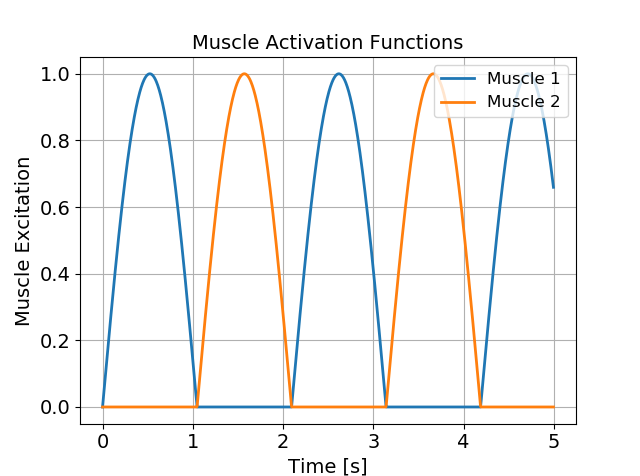
\includegraphics[width=.7\textwidth]{2b/2b_wave.png}
      \caption{Effect of Pendulum Angle on the Muscles}
      \label{fig:2bwave}
    \end{figure}
  
  %Activation = muscle stimulation right?
  With these waveform activating each muscle, the system was simulated and a phase plot of the results was created. To prove stability, Poincare analysis was performed. Figure \ref{fig:2bphase} shows the system, starting from initial conditions, then converging onto a limit cycle behaviour. The Poincare cross section is indicated on the plot. Figure \ref{fig:2bint} shows the intersection angles with the cross section for each crossing. While no clear convergence is shown, the scale of the values is within the margin of uncertainty of the model, given the integration methods and time-step used. Thus, it is fair to say that the system has indeed converged into a limit cycle behaviour. 
  
\begin{figure}[H]
    \centering
    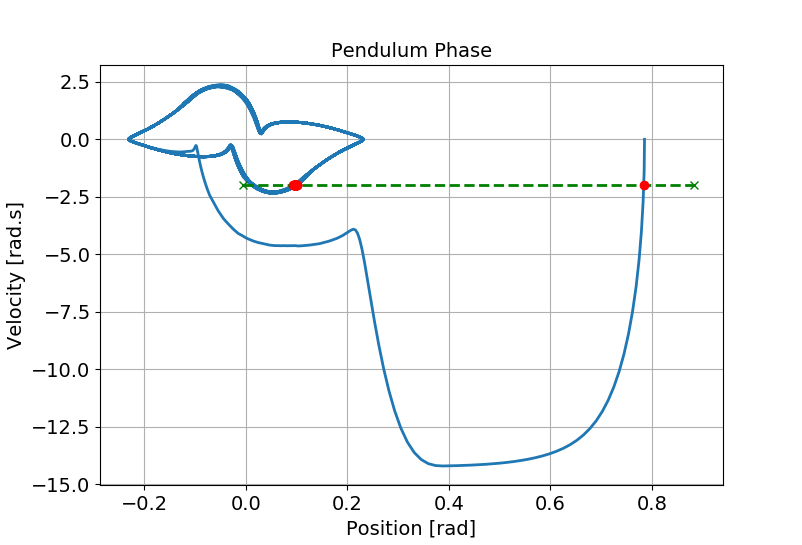
\includegraphics[width=0.6\textwidth]{2b/2b_phase.png}
    \caption{Pendulum Angle-Velocity Phase Plot showing limit cycle behaviour}
    \label{fig:2bphase}
\end{figure}

\begin{figure}[H]
    \centering
    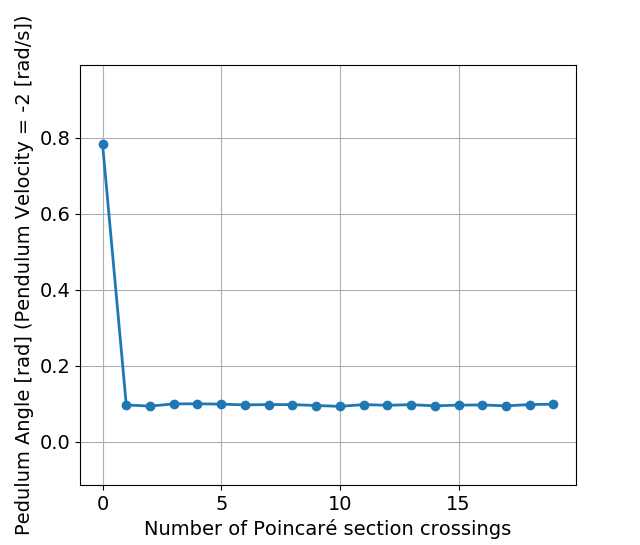
\includegraphics[width=0.6\textwidth]{2b/2b_pc_cross.png}
    \caption{Plot of the crossing location of each Poincare intersection point.}
    \label{fig:2bint}
\end{figure}

% Uncomment the following lines for a zoomed in version of the crossing points on the phase plot.     
%    \begin{figure}[H]
%      \centering
%      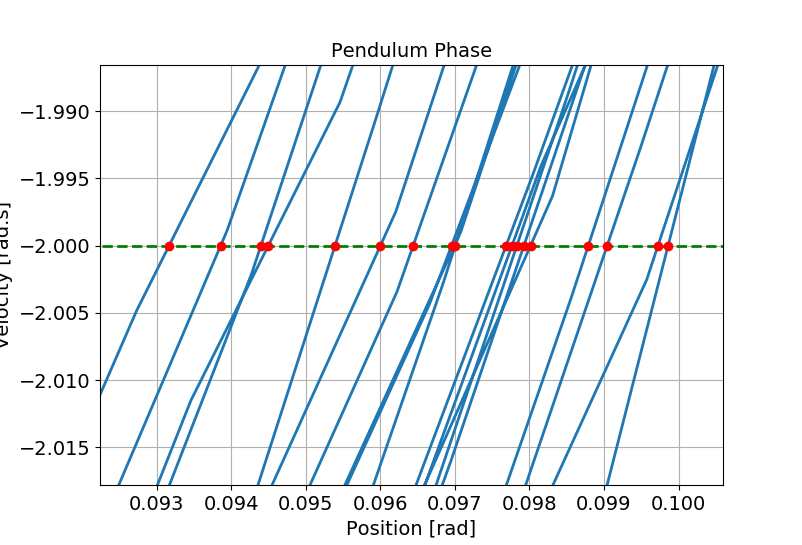
\includegraphics[width=\textwidth]{2b/2b_phase_zoomed.png}
%      \caption{Pendulum Angle-Velocity Phase Plot Zoomed-In Around Poincare Cross Section.}
%      \label{fig:2bzoom}
%    \end{figure}
  
\label{sec:2c}
\subsection*{2c. Show the relationship between stimulation frequency and amplitude with the resulting pendulum's behavior.}

To show the relationship between pendulum behaviour and the frequency and amplitude of muscle stimuli, the same half-sign wave functions used in Exercise 2b were used. However, in this experiment, the amplitudes and frequencies were varied. Amplitudes of 0.2, 0.5, and 1.0 were tested with a frequency of 3 rad/s. Then frequencies of 1, 2 and 3 rad/s were compared with an amplitude of 1. Figure \ref{fig:2c_Stimulation} shows the resultant phase-time relation from different configurations of stimulation. 

\begin{figure}[H]
    \centering
    \begin{subfigure}[t]{0.49\textwidth}
        \centering
        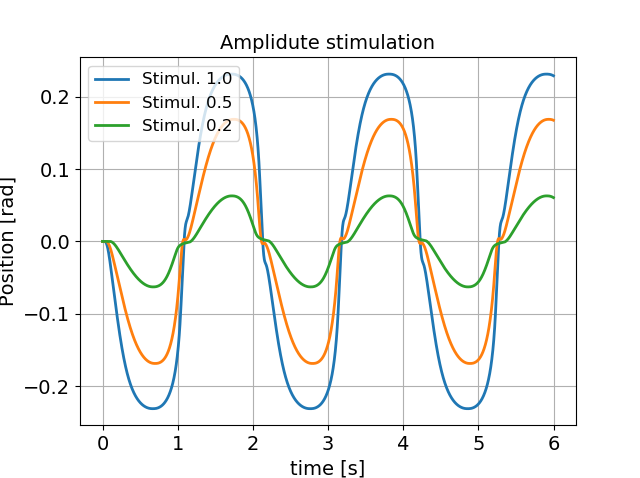
\includegraphics[width=\textwidth]{2c/2c_AmplitudeStimulation.png}
        \caption{Pendulum position over time, showing the effect of different stimulation amplitudes.}
    \end{subfigure}
    \hfill
    \begin{subfigure}[t]{0.49\textwidth}
        \centering
        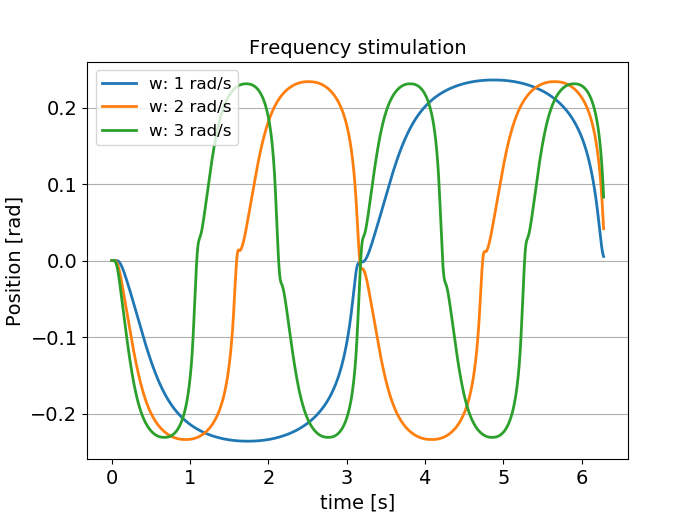
\includegraphics[width=\textwidth]{2c/2c_FrequencyStimulation.png}
        \caption{Pendulum position over time, showing the effect of different stimulation frequencies, where $\omega/ 2\pi = f$ [Hz], namely 0.159Hz, 0.318Hz and 0.477Hz.}
    \end{subfigure}
    \caption{Effect of different amplitude and frequency stimulation on the pendulum.}
    \label{fig:2c_Stimulation}
\end{figure}

The stimulation level largely determines the amplitude of the pendulum oscillations. As the muscle force is directly related to muscle stimulation, this makes intuitive sense. As the pendulum crosses the zero position, a concavity change can be noted in all plots. This change indicates the change in stimulation of the muscles at the point of peak muscle velocity. As the pendulum crosses through the 0 angle position, the active forces are zero, but the passive forces (particularly the parallel element) are unbalanced as their magnitude is dependent on the direction of the muscle velocity. Interestingly, in the case with full muscle stimulation, this concavity shift occurs at an angle higher than in the case of the small stimulation amplitude. This indicates a phase lag between the stimulation commands and the pendulum positioning.\\

Varying the stimulation frequency also yields interesting results. The lower frequency stimulation had the most pronounced concavity change at the zero crossing, but had the smallest phase lag of the 3 tested stimulation amplitudes. The duration of the concavity change is expected to be larger, simply due to the slower rate of change of muscle stimulation causing the slower movement of the pendulum. The phase lag increase with increased frequency is also expected, as the velocities involved are higher and the system's inertia plays a larger role. 

\newpage
\section*{Exercise 3 : Neural network driven pendulum model with
  muscles}
\label{sec:neur-netw-driv}

In this exercise, the goal is to drive the above system
\ref{fig:p_muscles} with a symmetric four-neuron oscillator
network. The network is based on Brown's half-center model with
fatigue mechanism. Here we use the leaky-integrate and fire neurons
for modelling the network. Figure \ref{fig:p_muscles_neurons} shows
the network structure and the complete system.

\begin{figure}[H]
  \centering
  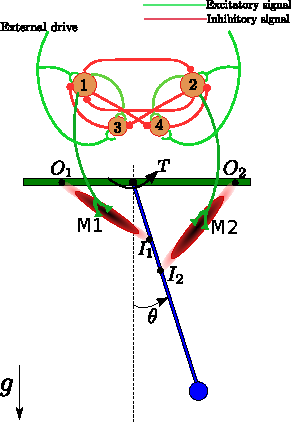
\includegraphics[scale=1.5]{figures/pendulum_muscles_neurons.pdf}
  \caption{Pendulum with Antagonist Hill Muscles Driven Half Center
    Neural Network.}
  \label{fig:p_muscles_neurons}
\end{figure}

Since each leaky-integrate and fire neuron comprises of one first
order differential equation, the states to be integrated now increases
by four(one state per neuron). The states are,


\begin{equation}
  \label{eq:7_lab6}
  X = \begin{bmatrix}
    \theta & \dot{\theta} & A_1 & l_{CE1} & A_2 & l_{CE2} & m_1 & m_2 & m_3 & m_4
  \end{bmatrix}
\end{equation}

Where,
\begin{itemize}
\item $m_1$ : Membrane potential of neuron 1
\item $m_2$ : Membrane potential of neuron 2
\item $m_3$ : Membrane potential of neuron 3
\item $m_4$ : Membrane potential of neuron 4
\end{itemize}

To complete this exercise, additionally you will have to use
\fileref{neural\_system.py} and \fileref{exercise3.py}

\subsection*{3a. Find a set of weights for the neural network that
  produces oscillations to drive the pendulum into a limit cycle
  behavior. Plot the output of the network and the phase plot of
the pendulum}
\label{sec:4a}

As seen in lecture \textit{"lecture4\_Neuron\_Models"}, the different weights of the neural network that cause the system to oscillate are as follows. These weights determine how the system of neurons inhibits and excites each other: 
\begin{eqnarray}
    w = \left[
        \begin{array}{rrrr}
            0 & -5 & -5 & 0 \\
            -5 & 0 & 0 & -5 \\
            5 & -5 & 0 & 0 \\
            -5 & 5 & 0 & 0
        \end{array}
    \right]
    \label{mat:neuron_weights}
\end{eqnarray}

By doing this, the neuronal network outputs become evident in an stable oscillatory pattern. Here the external excitation accordingly has value of zero. Figure \ref{fig:3a_NeuronSimulations} below shows the output of the neurons over time. In particular, the transient between each neuron's initial state and the final limit cycle can be seen between 0 and 0.2 seconds. 

\begin{figure}[H]
      \centering
      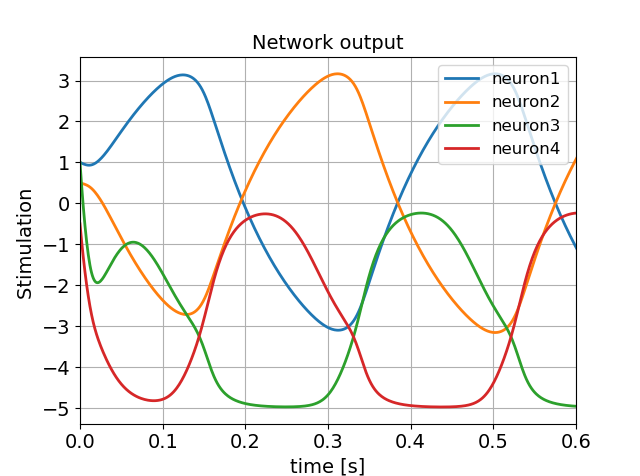
\includegraphics[width=.65\textwidth]{3a/3a-output.png}
      \caption{Neuron outputs over time during limit cycle behaviour.}
      \label{fig:3a_NeuronSimulations}
\end{figure}

Figure \ref{fig:3a_VelocityPhase} demonstrates the stability of the limit cycle with different initial conditions and disturbances. In each case, the system quickly returns to the limit cycle (purple colour). 

\begin{figure}[H]
      \centering
      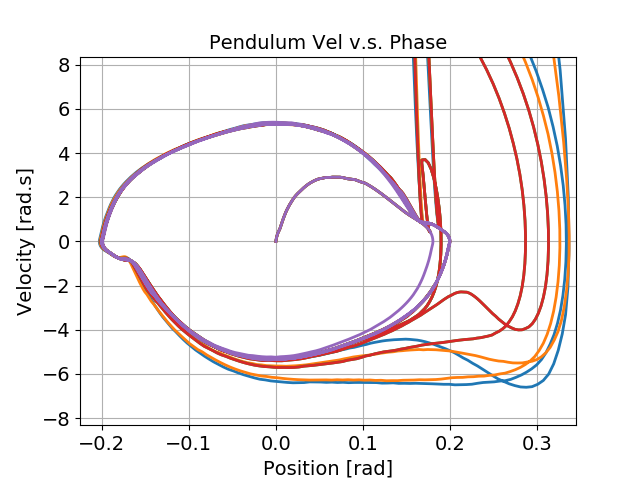
\includegraphics[width=.65\textwidth]{3a/3a_VelocityPhase.png}
      \caption{Limit cycle behaviour of a neural network controlled muscle-pendulum system. Different starting positions and disturbances are shown in different colors. All traces return to the same stable limit cycle.}
      \label{fig:3a_VelocityPhase}
\end{figure}

In Figure \ref{fig:3a_VelocityTime} some disturbances have been applied to the system in order to demonstrate that it will always go back to the limit cycle behavior. To obtain them, some runs were done with different disturbances (change in angular velocity, applying a torque or different initial conditions) and plot on the same graph to see the behaviour without disturbances. 
In the Phase graph all disturbances converge to the blue curve (line without dirturbances). In the Velocity graph all perturbations converge to the purple curve. So in all cases we achieve a limit cycle. 


\begin{figure}[H]
    \centering
    \begin{subfigure}[t]{0.48\textwidth}
        \centering
        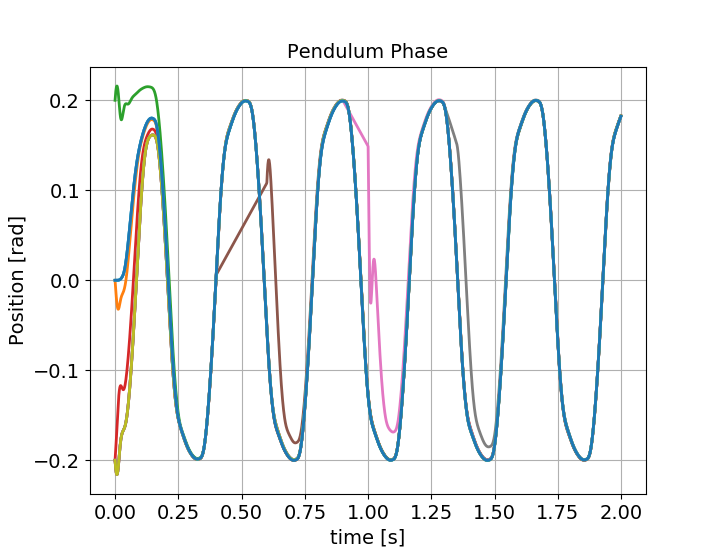
\includegraphics[width=\textwidth]{3a/3a_PhaseTimev.png}
        \caption{Pendulum position over time, showing the effect of different initial conditions and disturbance (angular speed and torque), shown in orange, green, brown, and pink. The blue one is the behavior without any disturbances.}
    \end{subfigure}
    \hfill
    \begin{subfigure}[t]{0.50\textwidth}
        \centering
        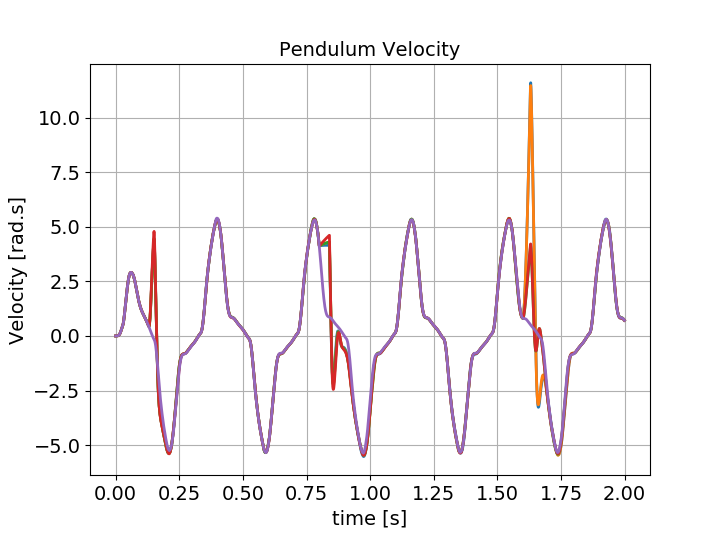
\includegraphics[width=\textwidth]{3a/3a_VelocityTimeii.png}
        \caption{Pendulum velocity over time, showing the effect of different disturbances (angular speed and torque), shown in orange, red and green. The violet one is the behavior without any disturbances.}
    \end{subfigure}
    \caption{Effect of disturbances on the pendulum.}
    \label{fig:3a_VelocityTime}
\end{figure}

\subsection*{3b. As seen in the course, apply an external drive to the
  individual neurons and explain how the system is affected. Show
  plots for low [0] and high [1] external drives. To add external
  drive to the network you can use the method \\
  \fileref{system\_simulation.py::add\_external\_inputs\_to\_network} }
\label{sec:4c}
%%%%%%%%%%%%%%%%%%%%%%%%%

For all Figures in this section there is a change in stimulation (from 0.0 to 1.0) of all neurons in the network at time 2 seconds. Observable is the increase in oscillating frequency of the pendulum, with a decrease in oscillating amplitude. 

\begin{figure}[H]
      \centering
      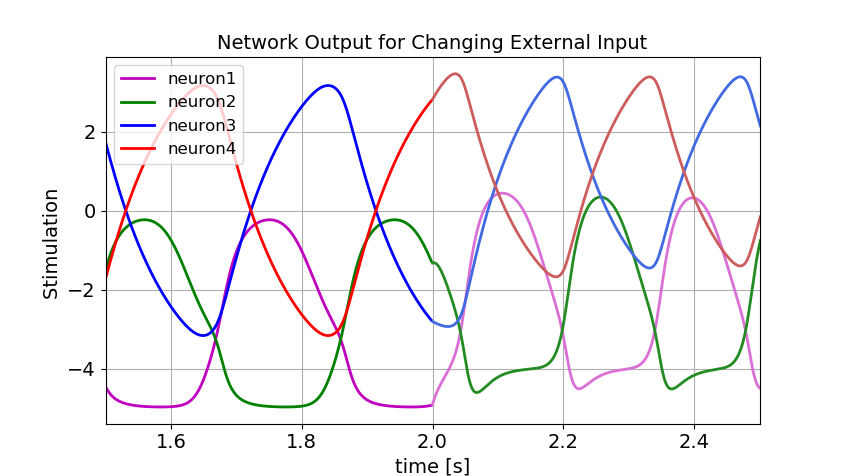
\includegraphics[width=.7\textwidth]{3b/3b-output.png}
      \caption{Effect of external inputs of 0.0 and 1.0 to the neurons}
      \label{fig:3b_NeuronSimulations}
\end{figure}

In the system we can observe the change in frequency and in amplitude of the system by applying external stimulation (t>2s). The transition between the two limit cycles, as shown in Figure \ref{fig:3b_VelocityPhaseSimulations} and \ref{fig:3b_VelocityTimeSimulations}, is smooth and the system resettles quickly.

\begin{figure}[H]
    \centering
    \begin{subfigure}[t]{0.5\textwidth}
        \centering
        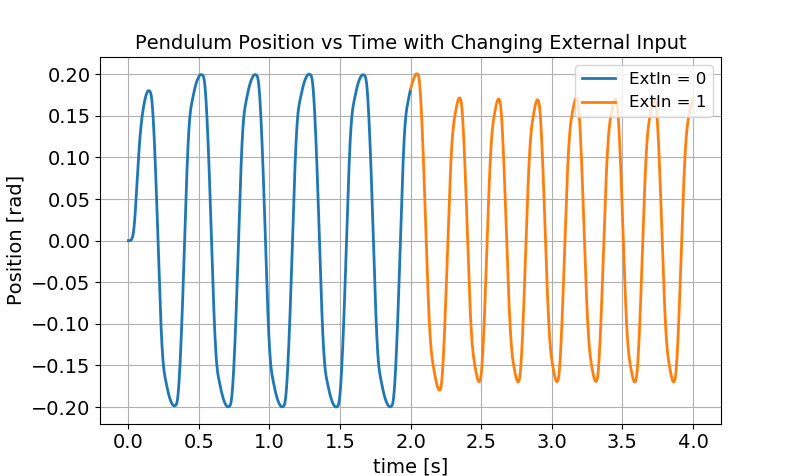
\includegraphics[width=\textwidth]{3b/3b-position.png}
        \caption{Pendulum Position over Time with and without External Input}
    \end{subfigure}
    \hfill
    \begin{subfigure}[t]{0.48\textwidth}
        \centering
        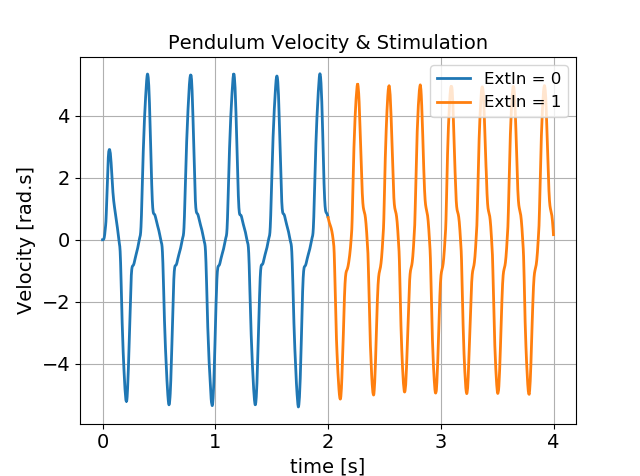
\includegraphics[width=\textwidth]{3b/3b-vel.png}
        \caption{Pendulum Velocity over Time with and without External Input}
    \end{subfigure}
    \caption{Effect of Pendulum Angle on the Muscles. at 2 seconds the stimulation changes to 1.0, producing a decrease on phase and angular velocities but an increase in frequency. }
    \label{fig:3b_VelocityTimeSimulations}
\end{figure}

\begin{figure}[H]
      \centering
      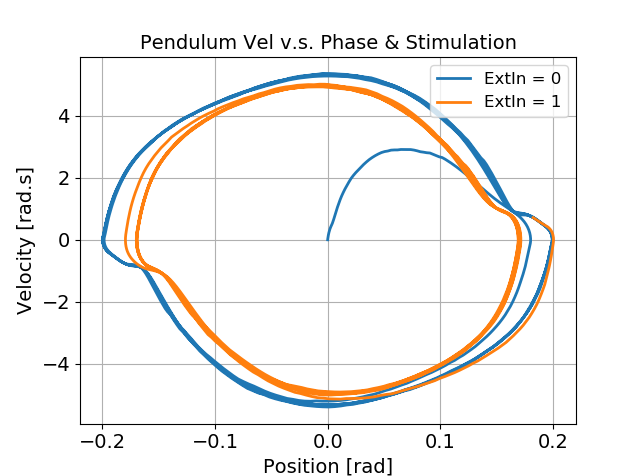
\includegraphics[width=.7\textwidth]{3b/3b-phase.png}
      \caption{Pendulum Phase Portrait before and after external input is introduced.}
      \label{fig:3b_VelocityPhaseSimulations}
\end{figure}

\subsection*{3c. [Open Question] What are the limitations of the half center model in producing alternating patterns to control the pendulum? What would be the effect of sensory feedback on this model? (No plots required)}
  
\subsubsection*{Limitations}
This model is idealized and is not robust to the severing of neuronal connections. If a connection is broken between two neurons it will not correctly react anymore. There is also no implementation of any reflexes so it can not well react to unexpected events or external disturbances. 

\subsubsection*{Sensory feedback}
The effect of sensory feedback on this model will result in a better imitation of the real behavior of the system and conduct to a more robust system because the neurons could be more implicate in the fine tuning of the parameters at each moment instead of also tune the stability. It will mainly improve when the mechanical characteristics are more like an over-damped system. In this case the strength of sensory feedback will be more important for the behavior than the mechanical properties.

It will also allow to know if the whole system is entirely functional or not by studying the feedback. This leads to redundancy and to have a more robust system. The reflexes of sensory feedback could also be implemented and avoid falling down on some situation like in the "Running over rough terrain" \footnote{"Running over rough terrain": guinea fowl maintain dynamic stability despite a large unexpected change in substrate height Monica A. Daley et al. J ExpBiol2006;209:171-187} paper where reflex give to the guinea fowl the capability of keeping its dynamic and do not falling down.
\end{document}

%%% Local Variables:
%%% mode: latex
%%% TeX-master: t
%%% End: